\documentclass[a4paper,ngerman]{scrartcl}

\usepackage{amsmath}
\usepackage{amsfonts}
\usepackage{amssymb}
\usepackage[utf8]{inputenc}
\usepackage{graphicx}
\usepackage[ngerman]{babel}
\usepackage{hyperref}
\usepackage{float}
\usepackage{caption}
\usepackage{subcaption}
\usepackage{multirow}  %for tables
\usepackage{icomma} % Handle german comma as decimal point in numbers
\usepackage{units,siunitx} % Write units with correct spacing
\usepackage{upgreek} % provide non-italic greek letters
\usepackage{url}
%\usepackage{subfig}

% Formatting of table & figure captions
\captionsetup{font={sf,footnotesize},labelfont=bf,textfont=sl,skip=6pt}
\setlength{\abovecaptionskip}{6pt}
\setlength{\belowcaptionskip}{0pt}

\title{Magnetisierung\\Versuchsvorbereitung}
\date{\today}
\author{Michel Rausch, Michael Eliachevitch}

\begin{document}

\maketitle
\tableofcontents
\newpage

\section{Einleitung}

%Versuchsbeschreibung:
%Es wird die Magnetisierung von Selten-Erd-Metallen (Tb, Gd)im Temperaturbereich T = 77 - 300 K bestimmt. 
%Dazu wird ein supraleitendes Quanteninterferometer (Superconducting Quantum-Interference Device, SQUID) aus einem Hochtemperatursupraleiter verwendet, das sich in einem Flüssigkstickstoff-gekühlten Dewar befindet.

Mit einem supraleitendem Quanteninterferometer, einem sogenanntem "'superconducting quantum interference device"' (\textbf{SQUID}) wird die Magnetisierung der Seltenen-Erde-Metalle Terbium (\textbf{Tb}) und Gadolinium (\textbf{SQUID}) bestimmt über einen Temperaturbereich von $T= \SI{77}{\kelvin} $ bis \SI{300}{\kelvin}.
Das SQUID wird mit flüssigem Stickstoff gekühlt und befindet sich daher in einem Dewar. 
In diesem Experiment werden die Grundlagen der Supraleitfähigkeit vertieft und in einer Messung angewandt.


\section{Theoretische Grundlagen}

\subsection{Supraleitung}

Supraleitung bezeichnet den Effekt, das einige Materialien, insbesondere Metalle, bei Unterschreitung einer Grenztemperatur $T_{\mathrm{C}}$ keinen Widerstand besitzen. 
Damit wird das Material diamagnetisch, Magnetfelder können nicht, oder nur gequantelt in den Supraleiter dringen. 
Beim Überschreiten von $T_{\mathrm{C}}$ bricht die Supraleitfähigkeit zusammen. 

Die technischen Anwendungsmöglichkeit sind weitreichend, jedoch meist in der Praxis durch $T_{\mathrm{C}}$ begrenzt, da die meisten Materialien mit flüssigem Helium gekühlt werden müssen. 
Andere Supraleiter, sogenannte Hochtemperatursupraleiter können mit flüssigem Stickstoff gekühlt werden, die bisher Entdeckten sind jedoch aus anderen Gründen ungeeignet.
Beispielsweise sind diese sehr spröde und daher für Drähte ungeeignet.




\subsection{Cooperpaare}

Für eine Supraleitungsfähigkeit müssen freie Elektronen vorhanden sein, daher tritt sie nur in Metallen auf.
Zusätzlich ist ein möglichst ideales Gitter nötig.
Die Elektronen im Material besitzen Energien entsprechend einer Fermistatistik.
Elektronen nahe der Fermikante können, aufgrund einer schwachen anziehenden Wechselwirkung, sogenannte \textbf{Cooper-Paare} bilden.
Das Cooper-Paar lässt sich mit einer gemeinsamen Wellenfunktion beschreiben. 
Um dieses zu stabilisieren helfen Gitterschwingen (\textit{Phononen}). 
Bei konventionellen Supraleitern ist der gepaarte Zustand energetisch günstiger, als der getrennte.
Es entsteht also eine Energielücke zwischen gepaarten und ungepaarten Elektronen. 

Die Stromdichte, bei der das Material widerstandsfrei leitet ist begrenzt durch die sogenannte \textbf{kritische Stromdichte}, die temperaturabhängig ist.
Hochtemperatursupraleiter sind noch nicht vollständig verstanden und werden daher aktuell erforscht.



\subsection{Supraleiter im Magnetfeld}

Supraleiter lassen sich kategorisieren anhand ihrer Wechselwirkung mit Magnetfeldern. Als \textbf{Supraleiter 1. Art} bezeichnet man solche, die das Magnetfeld vollständig verdrängen.  
Die meisten Supraleiter sind jedoch \textbf{2. Art}.
Sie verdrängen das Magnetfeld für geringe Feldstärken


\begin{figure}
\centering
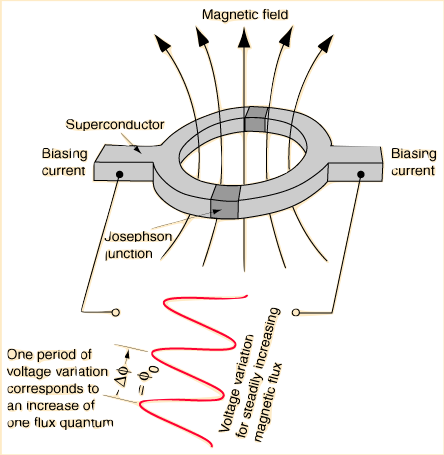
\includegraphics[width=0.7\textwidth]{abbildungen/squide.png}
\caption[Versuchsplatz]{\textbf{Flussfadengitter in einem Typ II-Supraleiter [\ref{ref:mappe}].}}
\label{fig:typII}
\end{figure}


\subsection{Meissner-Effekt}

\subsection{Josephson-Effekte}


\subsection{YBCO}

Das verwendete SQUID basiert auf Yttrium-Barium-Kupferoxid (\textbf{YBCO}). 


\section{Versuchsaufbau}

\subsection{SQUID}



\begin{figure}
\centering
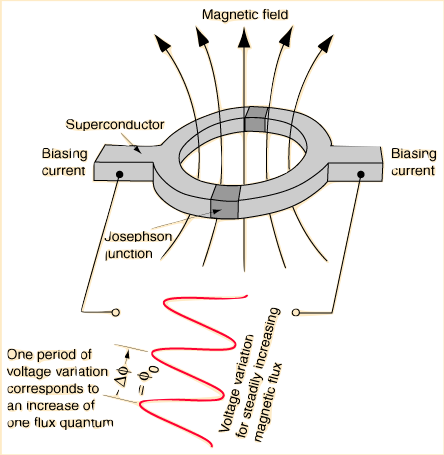
\includegraphics[width=0.7\textwidth]{abbildungen/squide.png}
\caption[Versuchsplatz]{\textbf{Aufbau eines SQUIDs [\ref{ref:wuppertal}].}}
\label{fig:squid_wuppertal}
\end{figure}

\subsubsection{Aufbau}

\subsubsection{Verhalten}

\subsection{Versuchsplatz}

\begin{figure}
\centering
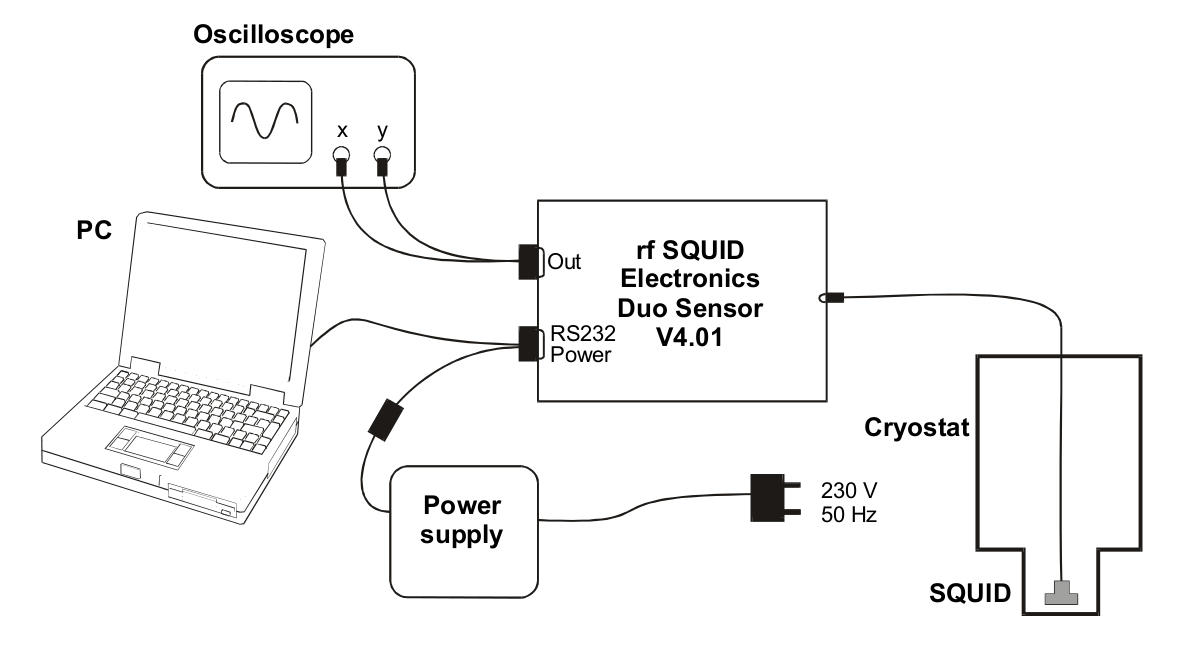
\includegraphics[width=0.7\textwidth]{abbildungen/aufbau_versuchsplatz.png}
\caption[Versuchsplatz]{\textbf{Aufbau des Versuchsplatz [\ref{ref:mappe}].}}
\label{fig:Versuchsplatz}
\end{figure}



\section{Versuchsdurchführung}


\section{Quellen}
\begin{enumerate}
\item Vorbereitungsmappe.\label{ref:mappe}
\item \url{http://hydrogen.physik.uni-wuppertal.de/hyperphysics/hyperphysics/hbase/solids/squid.html} ( 18.1.2015).\label{ref:wuppertal}
\end{enumerate}



\end{document}
